\chapter{Simulation Software}
\label{sec:hauptteil}
This chapter introduces the Sensor Network Tool Suite, highlighting its objectives and the collaborative efforts of IRAS, Fraunhofer FHR, and AIUB. The overview covers the five subprograms, 
including MWG, and outlines their roles in SSA programs through effective data processing and analysis.\\


\section{Introduction to the Sensor Network Tool suite}

To facilitate the advancement of SSA programs and effectively manage data from diverse databases, the creation of software capable of processing such information and supporting the evolution of networks 
and sensor technology was created. The Sensor Network Simulator(SNS) formerly known as Radar Systems Simulator (RSS) \cite{kebschull2017simulation}, commenced on January 1, 2015, with funding provided by DLR. The Institute of Space Systems (IRAS), in collaboration with the Fraunhofer
FHR, undertook the development of SNS. The primary objective of this project was to create a software solution dedicated to generating measurement data from sensors observing space debris, with a subsequent analysis and storage of this 
data in a database. Additionally, the results were to be systematically cataloged. The tool suite was implemented using the Fortran programming language.

Following the conclusion of the initial funding period, the program underwent renewal and recommenced in September 2018. During this phase, the Astronomical Institute of the University of Bern (AIUB) joined the Fraunhofer FHR in providing 
support to the IRAS for ongoing development efforts.

\subsection{Overview of the Program}

The complete tool suite comprises five distinct subprograms, each capable of independent use while synergistically complementing one another. Figure~\ref{fig:SNS} depicts the process flow within SNS and its subsystems.
Following are the tools used in the SNS software \cite{schubert2023enhancing} :

\begin{itemize}
    \item MWG (MessWertGenerator): Measurement value generation
    \item SMART (Sophisticated Module for the Analysis of Radar Tracklets): Orbit determination algorithms
    \item PROCOR (PROcess COoRdinator): Process coordination
    \item CAT (Catalog Analysis Tool): Catalog statistics
    \item CAMP (Catalog Maintenance and Pass prediction tool): Conjunction analysis and pass prediction
\end{itemize}

\begin{figure}[h!]
	\centering
	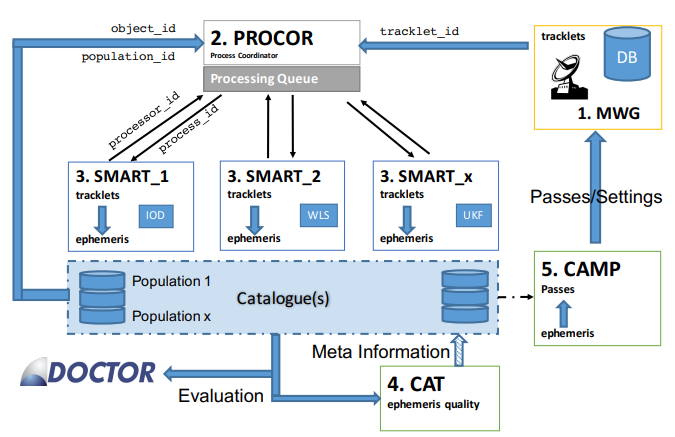
\includegraphics[width=0.9\textwidth]{SNS.png}
	\caption{A schematic representation of the process flow within the SNS \cite{kebschull2017simulation}}\label{fig:SNS}
\end{figure}

\subsubsection{MWG (Measurement Generation)}
MWG is responsible for generating synthetic measurements from radar sensors. It models the state of an object in terms of azimuth, elevation, range, and range-rate information. 
The tool supports different sensor modes such as Mechanical Tracking, Electronic Tracking, and Scanning, with configurable parameters including Field of View, beam opening angle, wavelength, power, antenna characteristics, 
and more. The Signal-to-Noise Ratio (SNR) is calculated, incorporating measurement uncertainties based on the derived SNR and a root-means-square error model. The software relies on the numerical propagator NPI 
Ephemeris Propagation Tool with Uncertainty Extrapolation (NEPTUNE) for object state extrapolation \cite{kebschull2017simulation}.

\subsubsection{SMART (Sophisticated Module for Analysis of Radar Tracklets)}
SMART processes tracklets and corresponding detectioons retrieved from the database using various Orbit Determination (OD) techniques. 
For Initial Orbit Determination (IOD), SMART supports the Gibbs and Herrick-Gibbs methods. For statistical OD, it employs Weighted Least Squares (WLS), Extended Kalman Filter (EKF), Unscented Kalman Filter (UKF), Preliminary orbit determination method documented in the Goddard Trajectory Determination System (GTDS),
Gauss iterative, Gooding, and Double-R angles-only methods, Cubature Kalman Filter (CKF), Ensemble Kalman Filter (EnKF), Gaussian Sum Kalman Filters (GS-UKF, GS-CKF) methods \cite{ams}. NEPTUNE propagator is utilized to extrapolate state and covariance from an object catalog to the measurement epoch. SMART can run in parallel with multiple instances, accessing the database and processing tracklets concurrently \cite{kebschull2017simulation}.

\subsubsection{PROCOR (Process Coordinator)}
PROCOR manages SMART instances and configures them using presets. It creates and distributes processes to running SMART instances, where each process involves applying OD algorithms 
to update or derive a new orbit. PROCOR ensures proper correlation of tracklets to objects in the catalog and selects configurations from the database based on the kind of orbit. These configurations encompass both OD and 
propagator settings, facilitating efficient handling of tasks and jobs \cite{kebschull2017simulation}.

\subsubsection{CAT (Catalogue Analysis Tool)}
CAT assesses the status of the object catalogue by deriving statistics on timeliness and accuracy. It monitors individual objects by comparing ephemeris data derived through OD algorithms 
in SMART to the truth known by MWG. CAT analyzes the difference between true and derived states, expressed in radial, along-track, and cross-track components. Additionally, it evaluates the covariance's ability to reflect 
uncertainties introduced during data measurement, extrapolation, and processing. CAT allows users to correlate data directly, including residuals, signal-to-noise ratio, and the orbital path during measurements. The Display 
of Object Circulating in Terrestrial Orbits (DOCTOR) program, integrated with CAT, visualizes objects in a 3D representation of Earth orbits \cite{kebschull2017simulation}.

\subsubsection{CAMP (Catalogue Maintenance and Pass prediction tool)}
The fifth tool in the sequence serves to establish a connection with the sensors. CAMP systematically reviews the object catalogue, generating pass predictions for objects that traverse the local horizon of registered sensor 
stations. These predictions are formulated based on estimated epoch, range, range-rate, azimuth, and elevation information. CAMP includes a mode allowing the anticipation of close approaches. The tool employs the numerical 
propagator NEPTUNE for its calculations \cite{kebschull2017simulation}.

\subsection{Setup of the Software}

The software operates on an IRAS server and is managed remotely, leveraging the server's superior hardware for significantly faster simulations compared to standard consumer-grade computers. The simulation utilizes 40 threads for computations, with a prudent restriction to 75 percent usage to allow ongoing server availability for other projects. Configuration settings in a file dictate simulation parameters.\\
Following are the conditions under which simulations were performed:\\
\begin{itemize}
	\item Sensor used : ESA Optical Ground Station, Spain
    \item Start of simulation: November 1, 2016, at 00:00:00 (UTC)
    \item End of simulation: November 3, 2016, at 00:00:00 (UTC)
    \item Length of one step in days: 0.025
    \item Lower diameter (m) limit, used for population filtering: 0.01
    \item Input file for telescope: telescope\_geo.sim (The input file contains objects in GEO)
\end{itemize}

\begin{lstlisting}[basicstyle=\ttfamily\footnotesize, language=TeX, caption={An excerpt from the input file ''telescope\_geo.sim''}]
#  Epoch: 2016-11-01 00:00 (YYYY-MM-DD HH:mm) (filtered) 
#  MASTER v8.0.0 Population run (quarterly epochs) 
# MASTER-Population for obects bigger than 1cm 
# Limits: m=[0.000,999999.000] | d=[0.100,9999999.000] | m/A=[0.000,999999.000] | a=[39000.000,46000.000] 
# | e=[0.000,0.300] | i=[0.000,180.000] | W=[0.000,360.000] | w=[0.000,360.000] | M=[0.000,360.000] 
#  Condensed population (all sources combined!) 
#  Identification label: 31 
023900001  1.0000E+00  3.7190E+00  1.0000E+00   6.677      43030.8  0.0264    7.07   305.83   296.63   140.04
023900002  1.0000E+00  5.4330E+00  8.9220E-01  12.260      42527.5  0.0266    6.82   305.58   135.89    48.28
023900003  1.0000E+00  8.4590E+01  8.1020E-01 231.623      43655.9  0.0167    7.31   306.18    37.53   290.20
023900004  1.0000E+00  2.8750E+00  7.4530E-01   9.307      43112.1  0.0083    7.35   305.58    84.91   205.82
023900005  1.0000E+00  1.9410E+00  6.9230E-01   7.283      42579.6  0.0179    7.49   304.85   142.65   182.04
023900006  1.0000E+00  1.6170E+00  6.4820E-01   6.923      39861.8  0.0996    5.97   303.03   171.76   326.80
023900007  1.0000E+00  5.4930E+00  6.1070E-01  26.507      42434.3  0.0141    6.49   305.91   169.25   321.50
023900008  1.0000E+00  1.0670E+00  5.7840E-01   5.740      42196.4  0.0358    7.30   304.61   146.20   239.77
023900009  1.0000E+00  1.4180E+00  5.5010E-01   8.438      42026.7  0.0252    7.19   304.53   173.28   241.35
023900010  1.0000E+00  1.5430E+00  5.2520E-01  10.074      43825.6  0.0227    6.62   307.25    50.89   325.63
023900011  1.0000E+00  1.5210E+00  5.0300E-01  10.826      42913.0  0.0173    7.85   304.84   116.90   156.32
023900012  1.0000E+00  1.1620E+01  4.8310E-01  89.664      42678.9  0.0116    7.36   305.10   145.15   161.47
023900013  1.0000E+00  8.5430E-01  4.6520E-01   7.114      43306.8  0.0233    6.50   306.89    92.02   291.45
\end{lstlisting}


\subsection{Implementation of the weighting schemes}

Having laid the theoretical groundwork regarding weighting schemes and the algorithm in the previous chapter, here specifics of the implementation of the weighting schemes along with the code snippets are given. 

\subsubsection{Implementation of weightings based on the time since last detection:}
The implementation involves calculating the time difference in hours since the last detection for each object. The calculated time difference is then used to determine the weight based on a defined time threshold. If the time since the last detection is less than the threshold, the weight is set to a value between 0 and 1, with a linear relationship to the elapsed time. Conversely, if the time exceeds the threshold, the weight is set to 0. This implementation ensures that objects with more recent detections receive higher weights, promoting effective sensor tasking and timely observation. Setting the threshold time to 72 hours has consistently demonstrated superior performance across multiple simulations, following experimentation with various values.\\

\begin{lstlisting}

! Here set the time threshold at which time the weight reaches 1.0
t_threshold = 72.0_dp
! Here we calculate the weight for each object based on the time since the last detection
do iObject = 1, size(tasking_objects)
	! Calculate the time difference in hours since the last detection
	time_since_last_detection = (objects(iObject)%ephemerides(1)%epoch%mjd - tasking_objects(iObject)%detections(tasking_objects(iObject)%num_detections)%time%mjd) * 24.0_dp
				
	! Applying the weighting scheme: weight is 1 if time < 24 hours, otherwise 0
	if (time_since_last_detection < 72.0_dp) then
		tasking_objects(iObject)%weight = min(1.0_dp, max(0.0_dp, time_since_last_detection / t_threshold))
	else
		tasking_objects(iObject)%weight = 0.0_dp
	end if

	! Assighning weights to the tasking_objects array
	weight_linear = tasking_objects(iObject)%weight 
end do

\end{lstlisting}




\subsubsection{Implementation of Weightings based on the number of detections:}
The implementation involves calculating the weight for each object by considering the number of detections it has accumulated. The minimum and maximum thresholds for the number of allowed detections are defined as `min\_threshold\_num\_detections` and `max\_threshold \_num\_detections`, respectively. For objects with 100 or fewer detections, the weight is set to 1.0, signifying a high priority for observation. Similarly, for objects with 300 or more detections, the weight is set to 0.0, indicating a lower priority. For objects with detections between 100 and 300, a linear interpolation is employed to gradually decrease the weight, reflecting a decreasing priority for observation as the number of detections increases. These particular threshold values are set after trying multiple simulations. These values offer the optimal performance. \\

\begin{lstlisting}

! Here we calculate the weight of each object based on the number of detections
! Define parameters for the minimum and maximum number of allowed detections
max_threshold_num_detections = 300.0_dp
min_threshold_num_detections = 100.0_dp

! Here we calculate the weight of each object based on the number of detections
do iObject = 1, size(tasking_objects)

	!Calculate the number of detections for the object
	num_detections = tasking_objects(iObject)%num_detections

	! Calculate the weight based on the number of detections
	if (num_detections <= min_threshold_num_detections) then
		! Objects with 100 or fewer detections should have a weight of 1.0
		tasking_objects(iObject)%weight = 1.0_dp
	elseif (num_detections >= max_threshold_num_detections) then
		! Objects with 300 or more detections should have a weight of 0.0
		tasking_objects(iObject)%weight = 0.0_dp
	else
		! Linear interpolation for objects with detections between 10 and 300
		tasking_objects(iObject)%weight = 1.0_dp - (real(num_detections - min_threshold_num_detections) /  real(max_threshold_num_detections - min_threshold_num_detections))
	end if

	weight_det = tasking_objects(iObject)%weight      
end do

\end{lstlisting}
